\newif\ifglobal

%%%%%%%%%%%%%%%%%%%%%%%
%%% Compile to view %%%
%%%%%%%%%%%%%%%%%%%%%%%

%%%%%%%%%%%%%%%%%%%%%%%%%%%%%%%%%%%%%%%%%%%%%%%%%%%
%%% Readme:                                     %%%
%%% https://www.overleaf.com/read/bwdjvfjksvjy/ %%%
%%%%%%%%%%%%%%%%%%%%%%%%%%%%%%%%%%%%%%%%%%%%%%%%%%%

% >>> M?: marks a module setting number or important notice

% >>> M4: Set {./relative-path} to external files for this module <<<
\def \modulefiles {./25-SENSOR}
% To add an external file, use:
% (Replace '---' with actual filename)
% '\input{\modulefiles/tables/---.tex}' for tables
% '\includegraphics{\modulefiles/figures/---}' for figures
% '\subfile{\modulefiles/---}' for register files


% >>> M1: This module is in global project? <<<
% 'YES' - uncomment; 'NO' - comment out
\globaltrue

\ifglobal
    \documentclass[main\_\_CN.tex]{subfiles}

\else
    % Font "FandolSong-Regular" used by ctex does not have GSUB table.
    % It causes warnings that do not affect compilation and can be ignored.
    \PassOptionsToPackage{quiet}{fontspec}

    \documentclass[openany, 10pt]{book}

    % >>> M2: In ./00-shared/preamble-trm-module, also find
    %         settings for visibility of todo notes, watermark <<<
    \usepackage{preamble-trm-module}


    % Enable Chinese typesetting
    \usepackage{ctex}

    % >>> M3: Temporary labels in Chinese
    %         you can add your own labels there <<<
    \myexternaldocument{./00-shared/temp-labels-cn}

\fi %\ifglobal


\setcounter{secnumdepth}{4}


% >>> M5: If this module needs any updates in
% './00-shared/preamble-trm-module.sty'
% (include additional package, etc.), contact your module PM
% or create the file './00-shared/changelog.tex' make the
% necessary updates yourself and document them in this file <<<


\begin{document}


% Sets language into which pre-defined bits of text are translated
\selectlanguage{chinese}

% Do not delete this block
\ifglobal
% Add the following front matter if
% this module is outside of global project
\else
    \InputIfFileExists{readme}{}{}
    {\let\clearpage\relax \listoftodos}
    {\let\clearpage\relax \listofdonetodos}
    \tableofcontents
    %\listoftables
    %\listoffigures
\fi


%%%%%%%%%%%%%%%%%%%%%%%%%
%%% TRM Module Begins %%%
%%%%%%%%%%%%%%%%%%%%%%%%%

\hypertarget{sensor}{}
\chapter{片上传感器与模拟信号处理}
\label{mod:sensor}

\section{概述}

\chipname{} 搭载了以下模拟信号处理设备和片上传感器：

\begin{itemize}
    \item 一个 12 位逐次逼近型模拟数字转换器 (SAR ADC)，支持五个通道的模拟信号检测；
    \item 一个温度传感器：用于测量 \chipname{} 芯片内部温度。

\end{itemize}

\section{SAR ADC}\label{sec:saradc}

\subsection{概述}

\chipname{} 内置了一个 12 位的 SAR ADC，可测量最多来自五个管脚的模拟信号。SAR ADC 由 DIG ADC 控制器控制。DIG ADC 控制器可驱动 \hyperref[block:digital-reader0]{Digital\_Reader} 分别对 SAR ADC 的通道电压进行采样，支持多通道扫描和阈值监控。

\subsection{特性}

SAR ADC 具有如下特性：

\begin{itemize}
\item SAR ADC 有专用的 ADC Reader 模块 Digital\_Reader 获取采样结果
\item 支持 12 位采样分辨率
\item 支持采集最多 5 个管脚上的模拟电压

\item DIG ADC 控制器：
    \begin{itemize}
        \item 配有单次采样和多通道扫描控制模块，分别支持单次采样模式和多通道扫描模式
        \item 支持单次采样模式和多通道扫描模式同时工作
        \item 在多通道扫描模式下，支持自定义扫描通道顺序
        \item 提供两个滤波器，滤波系数可配
        \item 支持阈值监控，采样值大于设置的高阈值或小于设置的低阈值将产生中断
    \end{itemize}
\end{itemize}


\subsection{功能描述}

SAR ADC 的主要元件与连接情况见图 \ref{fig:sar-adc-functional-overview}。
\begin{figure}[H]
    \centering
    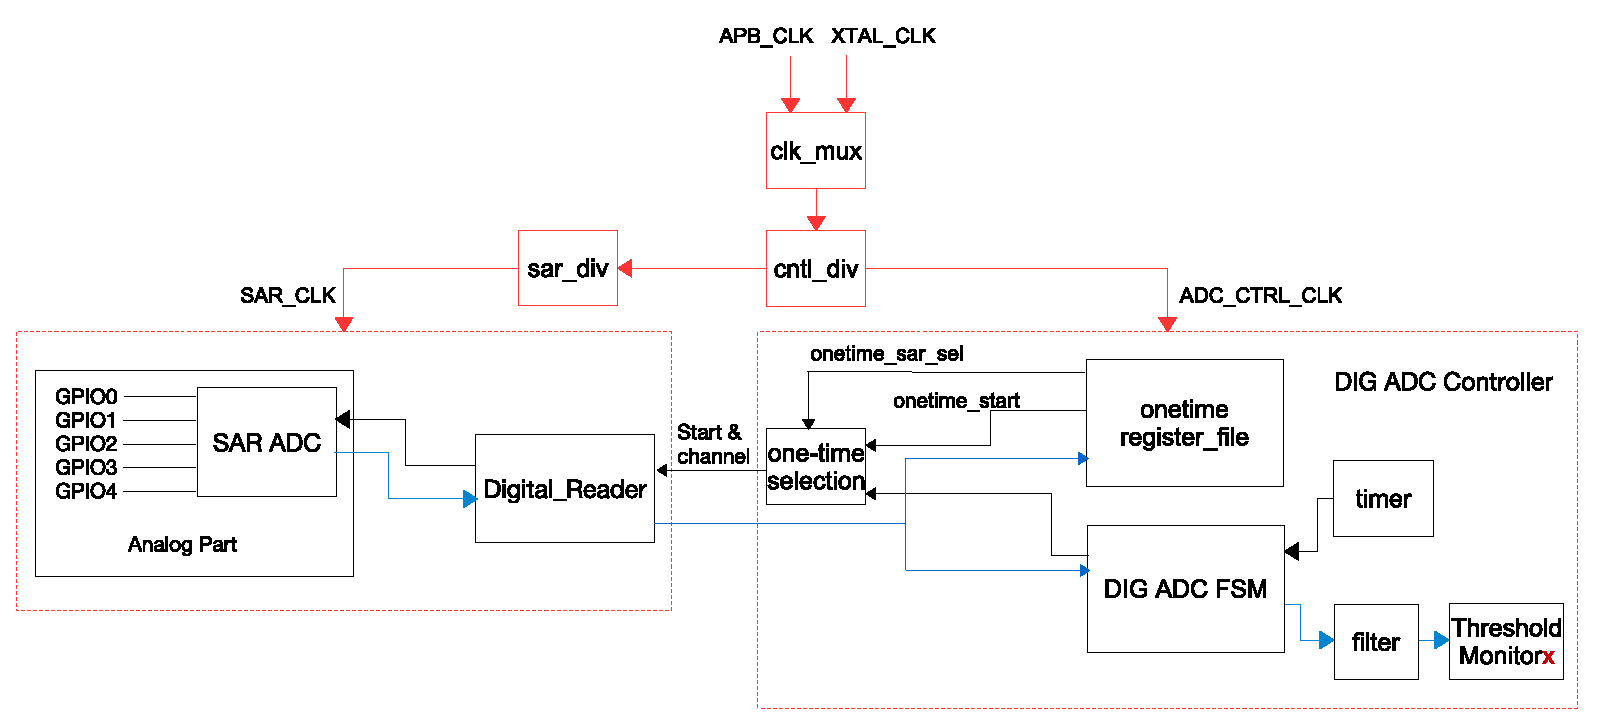
\includegraphics[width=1.0\textwidth]{./25-SENSOR/figures/on_chip_sensor_0926}
    \textcolor{blue}{\textbf{——>}}：数据流；\textcolor{red}{\textbf{——>}}：时钟信号；\textcolor{black}{\textbf{——>}}：控制信号
    \caption{SAR ADC 的功能概况}
    \label{fig:sar-adc-functional-overview}
\end{figure}

如图 \ref{fig:sar-adc-functional-overview} 所示，SAR ADC 模块主要包括以下元件：

\begin{itemize}
    \item SAR ADC：可对五个通道进行电压检测；
    \item 时钟管理：对时钟源进行选择和分频：
        \begin{itemize}
            \item 时钟源：可选择 APB\_CLK 或 XTAL\_CLK；
            \item 分频时钟：
             \begin{itemize}
                 \item SAR\_CLK：SAR ADC 和 Digital\_Reader 的工作时钟；其中控制 SAR\_CLK 分频的 sar\_div 的分频系数至少是 2 分频；
                 \item ADC\_CTRL\_CLK：DIG ADC FSM 的工作时钟。
             \end{itemize}
        \end{itemize}
    \item \label{block:digital-reader0} Digital\_Reader：由 DIG ADC FSM 驱动，读取 SAR ADC 的数值；
    \item DIG ADC FSM：生成整个 ADC 采样过程中所需的各种信号，下文简称 FSM。
    \item Threshold Monitor\regindex{x}：阈值监控器 1 和阈值监控器 2。可在采样值大于设定的高阈值，或小于设定的低阈值时触发中断。
\end{itemize}
以下小节将详细介绍各个元件。

\subsubsection{输入信号}

SAR ADC 需首先通过内部多路器选择待测量的模拟管脚，然后才能采样模拟信号。表 \ref{tab:adc-inputs} 列出了所有可能需要经过 SAR ADC 处理的模拟信号。

\begin{table}[H]
    \centering
    \caption{SAR ADC 的信号输入}
    \label{tab:adc-inputs}
    \begin{tabular}[c]{|p{3cm}|p{1.5cm}|}
    \hline
    \rowcolor{lightgray}
    \textbf{信号名称} & \textbf{通道编号} \\
    \hline
    GPIO0       &  0  \\\hline
    GPIO1       &  1  \\\hline
    GPIO2       &  2  \\\hline
    GPIO3       &  3  \\\hline
    GPIO4       &  4  \\\hline
\end{tabular}
\end{table}

\subsubsection{ADC 转换和衰减}

SAR ADC 转换模拟信号时，转换分辨率（12 位）电压范围为 0 mV \verb+~+ \(V_{ref}\)。其中，\(V_{ref}\) 为 SAR ADC 内部参考电压，出厂设定为 1100 mV。因此，转换结果 (data) 可以使用以下公式转换成模拟电压输出 \(V_{data}\)：

    \[
    V_{data} = \frac{V_{ref}}{k}\times{\frac{data}{4095}}
    \]

其中 k 为衰减对应的系数。

如需转换大于 \(V_{ref}\) 的电压，信号输入 SAR ADC 前可进行衰减。支持的衰减等级包括：

\begin{itemize}
    \item 0 dB (k≈100\%)
    \item 2.5 dB (k≈75\%)
    \item 6 dB (k≈50\%)
    \item 12 dB (k≈25\%)
\end{itemize}

\subsubsection{DIG ADC 控制器}


DIG ADC 控制器使用快速时钟，实现了采样速率大幅提升。该控制器最高支持 12 位采样分辨率，同时支持软件触发的单次采样和专用定时器触发的多通道扫描。更多参数和性能信息见\href{https://www.espressif.com/sites/default/files/documentation/esp8684_datasheet_en.pdf}{《\chipname{} 系列芯片技术规格书》}中的 ADC 特性章节。

软件驱动的单次采样的具体配置如下：
\begin{itemize}
    \item 置位 \hyperref[fielddesc:APBSARADCSARADC1ONETIMESAMPLE]{APB\_SARADC1\_ONETIME\_SAMPLE} 选择对 SAR ADC 进行单次采样；
    \item 配置 \hyperref[fielddesc:APBSARADCSARADCONETIMECHANNEL]{APB\_SARADC\_ONETIME\_CHANNEL} 选择采样通道；
    \item 配置 \hyperref[fielddesc:APBSARADCSARADCONETIMEATTEN]{APB\_SARADC\_ONETIME\_ATTEN} 选择衰减；
    \item 配置 \hyperref[fielddesc:APBSARADCSARADCONETIMESTART]{APB\_SARADC\_ONETIME\_START} 启动单次采样；
    \item 采样结束即触发 \hyperref[fielddesc:APBSARADCAPBSARADC1DONEINTRAW]{APB\_SARADC\_ADC1\_DONE\_INT\_RAW} 中断。软件检测该中断后，可在 \hyperref[fielddesc:APBSARADCAPBSARADC1DATA]{APB\_SARADC\_\\ADC1\_DATA} 寄存器内读到采样值。
\end{itemize}

如果选择专用定时器驱动的多通道扫描，可采用如下配置。注，在多通道扫描模式下，扫描序列可根据样式表的描述进行，样式表可配置。
\begin{itemize}
        \item 配置 \hyperref[fielddesc:APBSARADCSARADCTIMERTARGET]{APB\_SARADC\_TIMER\_TARGET} 设置 DIG ADC 定时器的触发周期。当定时器计数到配置周期数的 2 倍时，触发采样。定时器的工作时钟见章节 \ref{sec:dig-adc-clock}；
        \item 配置 \hyperref[fielddesc:APBSARADCSARADCTIMEREN]{APB\_SARADC\_TIMER\_EN} 使能定时器；
        \item 定时器超时则将驱动 DIG ADC FSM 根据样式表进行采样；
        \item \textbf{每次采样完成均会有中断产生，需要软件从对应寄存器中获取，否则采样数据经过阈值监控器之后将被直接丢弃。}
\end{itemize}


\subsubsection{DIG ADC 时钟}\label{sec:dig-adc-clock}

用户可配置 \hyperref[fielddesc:APBSARADCCLKSEL]{APB\_SARADC\_CLK\_SEL} 选择 DIG ADC 控制器的工作时钟：
\begin{itemize}
    \item 1：选择 XTAL\_CLK 的分频时钟 ADC\_CTRL\_CLK；
    \item 0：选择 APB\_CLK。
\end{itemize}

如果选择使用 ADC\_CTRL\_CLK，用户可配置 \hyperref[fielddesc:APBSARADCCLKMDIVNUM]{APB\_SARADC\_CLKM\_DIV\_NUM} 选择分频系数。

注意，由于 SAR ADC 有速度限制，所以 Digital\_Reader 和 SAR ADC 的工作时钟是 SAR\_CLK。SAR\_CLK 频率会影响采样精度，频率越低采样精度越高。SAR\_CLK 由 ADC\_CTRL\_CLK 经过专用分频器分频所得。分频系数通过 \hyperref[fielddesc:APBSARADCSARADCSARCLKDIV]{APB\_SARADC\_SAR\_CLK\_DIV} 配置。

ADC 每采样一个数据需要 25 个 SAR\_CLK 时钟周期数，所以最大采样速率受到 SAR\_CLK 的频率限制。更多时钟信息，见章节 \ref{mod:resclk} \textit{\nameref{mod:resclk}}。

\subsubsection{DIG ADC FSM}
\textbf{概述}

图 \ref{fig:dig-adc-overview} 展示了 DIG ADC FSM 的工作原理。
\begin{figure}[H]
    \centering
    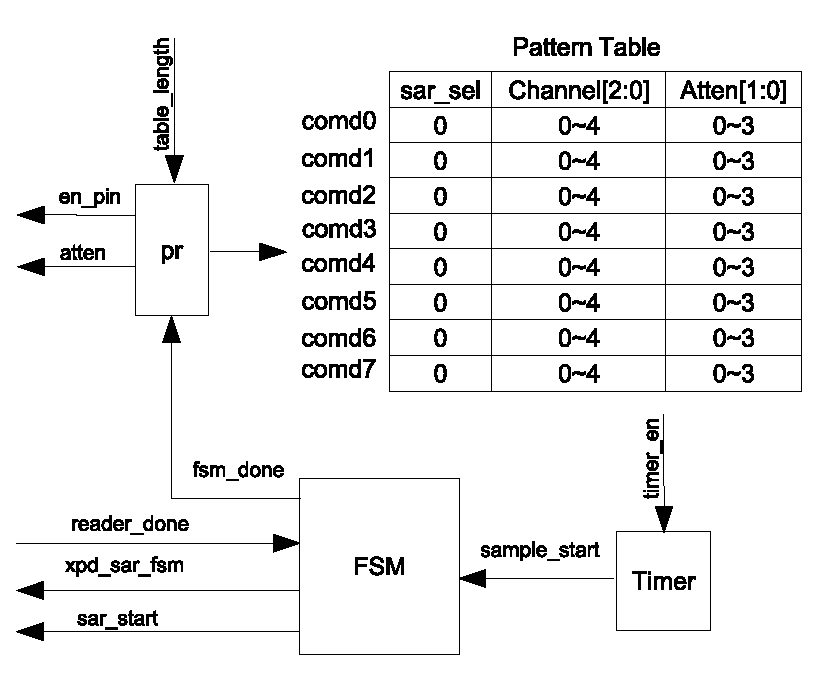
\includegraphics[width=0.6\textwidth]{./25-SENSOR/figures/dig_adc_fsm_overview_20221009}
    \caption{DIG ADC FSM 概况}
    \label{fig:dig-adc-overview}
\end{figure}
其中，
\begin{itemize}
    \item Timer：表示 DIG ADC 的专用定时器，可产生 sample\_start 信号；
    \item pr：样式表指针，FSM 将根据该指针指向的样式配置，发送相应信号。
\end{itemize}

相关执行过程如下：
\begin{itemize}
\item 置位 \hyperref[fielddesc:APBSARADCSARADCTIMEREN]{APB\_SARADC\_TIMER\_EN} 使能 DIG ADC 的专用定时器。定时器超时将触发 sample\_start 信号驱动 FSM 模块开始采样；
\item FSM 模块收到 sample\_start 信号后，执行以下操作：
\begin{itemize}
    \item 开启 SAR ADC 电源；
    \item 根据当前 pr 指向的样式，选择 SAR ADC 用作工作 ADC，同时配置 ADC 通道以及衰减；
    \item 根据配置信息，输出相应的 en\_pad（使能管脚）以及 atten（衰减）信号到模拟端；
    \item 发起 sar\_start 信号，开启采样。
\end{itemize}

    \item FSM 收到 Digital\_Reade 返回的 reader\_done 信号后，
    \begin{itemize}
        \item 结束采样；
        \item 数据传输给滤波器 (filter) 和阈值监控器 (threshold monitor) 后丢失（见图 \ref{fig:sar-adc-functional-overview}）；
        \item 更新样式表指针 pr，等待下一次采样。注意，如果指针 pr 小于 \hyperref[fielddesc:APBSARADCSARADCSARPATTLEN]{APB\_SARADC\_SAR\_PATT\_LEN} (table\_length)，则 pr = pr + 1；否则 pr 将被清零。
    \end{itemize}
\end{itemize}

\textbf{样式表结构}

DIG ADC FSM 包含一个样式表，由 \hyperref[regdesc:APBSARADCSARPATTTAB1REG]{APB\_SARADC\_SAR\_PATT\_TAB1\_REG} 和 \hyperref[regdesc:APBSARADCSARPATTTAB1REG]{APB\_SARADC\_SAR\_PATT\_TAB2\\\_REG} 两个寄存器组成，如图 \ref{fig:pattern-tab-1} 和图 \ref{fig:pattern-tab-2} 所示：

\regfield{(reserved)}{8}{24}{00000000}%
\regfield{cmd0}{6}{18}{{0x0000}}%
\regfield{cmd1}{6}{12}{{0x0000}}%
\regfield{cmd2}{6}{6}{{0x0000}}%
\regfield{cmd3}{6}{0}{{0x0000}}%
\begin{regdesc}\begin{reglist}
\item [cmd \regindex{x}] 表示样式表中的样式，即样式 0 \verb+~+ 样式 3。
\end{reglist}\end{regdesc}
\vspace{-2em}
\begin{figure}[H]
    \centering
    \caption{APB\_SARADC\_SAR\_PATT\_TAB1\_REG 与样式 0 - 3}
    \label{fig:pattern-tab-1}
\end{figure}

\regfield{(reserved)}{8}{24}{00000000}%
\regfield{cmd4}{6}{18}{{0x0000}}%
\regfield{cmd5}{6}{12}{{0x0000}}%
\regfield{cmd6}{6}{6}{{0x0000}}%
\regfield{cmd7}{6}{0}{{0x0000}}%
\begin{regdesc}\begin{reglist}
\item [cmd \regindex{x}] 表示样式表中的样式，即样式 4 \verb+~+ 样式 7。
\end{reglist}\end{regdesc}
\vspace{-2em}
\begin{figure}[H]
    \centering
    \caption{APB\_SARADC\_SAR\_PATT\_TAB2\_REG 与样式 4 - 7}
    \label{fig:pattern-tab-2}
\end{figure}

每个寄存器包含四个样式，每个样式长度为六位，共包括三个字段，分别存储了选择的工作 ADC、通道和衰减信息，具体见表 \ref{tab:pattern-table-register}。

\begin{figure}[H]
\centering
\regfield{sar\_sel}{1}{5}{{x}}%
\regfield{ch\_sel}{3}{2}{{xx}}%
\regfield{atten}{2}{0}{xx}%
\end{figure}
\vspace{-2em}
\begin{figure}[H]
    \centering
    \caption{样式表中的样式结构}
    \label{tab:pattern-table-register}
\end{figure}
\vspace{-2em}
\begin{regdesc}\begin{reglist}
\item [atten] 衰减配置信息。0：0 dB；1：2.5 dB；2：6 dB；3：10 dB。
\item [ch\_sel] 扫描通道选择信息，更多信息见表 \ref{tab:adc-inputs}。
\item [sar\_sel] ADC 选择信息。\chipname{} 只有一个 ADC，因此该位只能配置为 0。
\end{reglist}\end{regdesc}

\textbf{多通道扫描配置示例}

例如，希望实现如下所示的多通道扫描方式：
\begin{itemize}
    \item 扫描通道 2，且衰减配置为 10 dB；
    \item 扫描通道 0，且衰减配置为 2.5 dB。
\end{itemize}

则具体的配置如下：
\begin{itemize}
    \item 配置第一个样式 cmd0，如下图所示：

\centering
\regfield{sar\_sel}{1}{5}{{0}}%
\regfield{ch\_sel}{3}{2}{{2}}%
\regfield{atten}{2}{0}{3}%
\reglabel{}\regnewline%
\begin{regdesc}\begin{reglist}
\begin{figure}[H]
    \centering
    \caption{cmd0 配置示例}
\end{figure}
\vspace{-2em}
\item [atten] 配置该字段的值为 3，即衰减配置为 10 dB。
\item [ch\_sel] 配置该字段的值为 2，即选择通道 2（见表 \ref{tab:adc-inputs}）。
\item [sar\_sel] 配置该位为 0。
\end{reglist}\end{regdesc}
\end{itemize}

\begin{itemize}
    \item 配置第二个样式 cmd1，如下图所示：

\centering
\regfield{sar\_sel}{1}{5}{{0}}%
\regfield{ch\_sel}{3}{2}{{0}}%
\regfield{atten}{2}{0}{1}%
\reglabel{}\regnewline%
\begin{regdesc}\begin{reglist}
\begin{figure}[H]
    \centering
    \caption{cmd1 配置示例}
\end{figure}
\vspace{-2em}
\item [atten] 配置该字段的值为 1，即衰减配置为 2.5 dB。
\item [ch\_sel] 配置该字段的值为 0，即选择通道 0（见表 \ref{tab:adc-inputs}）。
\item [sar\_sel] 配置该位为 0。
\end{reglist}\end{regdesc}
\end{itemize}

\begin{itemize}
    \item 配置 \hyperref[fielddesc:APBSARADCSARADCSARPATTLEN]{APB\_SARADC\_SAR\_PATT\_LEN} 为 1，即选择使用上述配置好的样式表 0 和样式表 1；
    \item 使能定时器，则 DIG ADC 控制器将根据上述样式配置，周期性采样通道 2 和通道 0。
\end{itemize}


\subsubsection{ADC 滤波器}
DIG ADC 控制器支持滤波功能，提供两个滤波器。两个滤波器均可配置 SAR ADC 的任一通道，然后对目标通道的采样数据进行滤波。滤波公式如下所示：

\[data_{cur} = \frac{(k-1)data_{prev}}{k}+\frac{data_{in}}{k}+0.5\]

\begin{itemize}
    \item \(data_{cur}\)：滤波后数据
    \item \(data_{in}\)：ADC 采样值
    \item \(data_{prev}\)：上次滤波数据
    \item \(k\)：滤波系数
\end{itemize}

配置滤波器如下：
\begin{itemize}
\item 配置 \hyperref[fielddesc:APBSARADCAPBSARADCFILTERCHANNEL1]{APB\_SARADC\_FILTER\_CHANNEL\regindex{x}} 设置滤波器 \regindex{x} 作用的 ADC 通道
\item 配置 \hyperref[fielddesc:APBSARADCAPBSARADCFILTERCHANNEL1]{APB\_SARADC\_FILTER\_FACTOR\regindex{x}} 设置滤波器 \regindex{x} 的滤波系数
\end{itemize}

注意，这里的 \regindex{x} 为滤波器编号：\regindex{x} 为 0 表示滤波器 \regindex{0}；为 1 表示滤波器 \regindex{1}。

\subsubsection{阈值监控}
DIG ADC 控制器包含两个阈值监控器，可配置到 SAR ADC 的任意通道上。当 ADC 采样值大于设定的高阈值，则触发高阈值中断；若采样值小于设定的低阈值，则触发低阈值中断。

阈值监控配置如下：
\begin{itemize}
    \item 配置 \hyperref[fielddesc:APBSARADCAPBSARADCTHRES1EN]{APB\_SARADC\_THRES\regindex{x}\_EN} 使能阈值监控 \regindex{x} 的功能；
    \item 配置 \hyperref[fielddesc:APBSARADCAPBSARADCTHRES1LOW]{APB\_SARADC\_THRES\regindex{x}\_LOW} 设置低阈值；
    \item 配置 \hyperref[fielddesc:APBSARADCAPBSARADCTHRES1LOW]{APB\_SARADC\_THRES\regindex{x}\_HIGH} 设置高阈值；
    \item 配置 \hyperref[fielddesc:APBSARADCAPBSARADCTHRES1LOW]{APB\_SARADC\_THRES\regindex{x}\_CHANNEL} 设置监控的通道。
\end{itemize}

注意，这里的 \regindex{x} 为阈值监控器编号：\regindex{x} 为 0 表示阈值监控器 \regindex{0}；为 1 表示阈值监控器 \regindex{1}。



\section{温度传感器}\label{sec:tsensor}
\subsection{概述}
\chipname{} 搭载了温度传感器可以实时监测芯片内部温度。

\subsection{特性}
温度传感器的主要特性包括：
\begin{itemize}
    \item 支持软件触发，且一旦触发后，可持续读取数据
    \item 可根据使用环境配置温度偏移，提高测试精度
    \item 测量范围可调节
\end{itemize}


\subsection{功能描述}

温度传感器可由软件启动，具体配置如下：
    \begin{itemize}
        \item 置位 \hyperref[fielddesc:APBSARADCTSENSPU]{APB\_SARADC\_TSENS\_PU}，温度传感器上电；
        \item 等待 \hyperref[fielddesc:APBSARADCTSENSXPDWAIT]{APB\_SARADC\_TSENS\_XPD\_WAIT} 个时钟周期后，温度传感器的复位释放，开始测量环境温度；
        \item 首次开启温度传感器，需要等待一定的启动时间（大致为 100 $\mu$s），之后可以从 \hyperref[fielddesc:APBSARADCTSENSOUT]{APB\_SARADC\_TSENS\_OUT} 中即可持续获取温度值。
    \end{itemize}

温度传感器的输出值需要使用转换公式转换成实际的温度值(°C)。转换公式如下：
\[
        T(°C) = 0.4386 * VALUE – 27.88 * offset – 20.52
\]

其中 VALUE 即温度传感器的输出值，offset 由温度偏移决定。 温度传感器在不同的实际使用环境（测量温度范围）下，温度偏移不同，见表 \ref{tab:tsensor-dac}。

\begin{longtable}[c]{|p{4cm}|p{4cm}|}
    \caption{温度传感器的温度偏移}
    \label{tab:tsensor-dac}
    \\\hline
    \rowcolor{lightgray}
    测量范围 (°C)  & 温度偏移 (°C) \\\hline
    50 \verb+~+ 125 & -2 \\\hline
    20 \verb+~+ 100 & -1 \\\hline
    -10 \verb+~+ 80 & 0 \\\hline
    -30 \verb+~+ 50 & 1 \\\hline
    -40 \verb+~+ 20 & 2 \\\hline
\end{longtable}

\section{中断}

\begin{itemize}
   \item \label{interreupt:SARADCDONEINT1} APB\_SARADC\_ADC1\_DONE\_INT：SAR ADC 完成一次转换，即触发此中断；
   \item \label{interreupt:APBSARADCTHRESxHIGHINT} APB\_SARADC\_THRES\regindex{x}\_HIGH\_INT：超过阈值监控器 \regindex{x} 的高阈值，即触发此中断；
    \item \label{interreupt:APBSARADCTHRESxLOWINT} APB\_SARADC\_THRES\regindex{x}\_LOW\_INT：低于阈值监控器 \regindex{x} 的低阈值，即触发此中断。
\end{itemize}

\section{寄存器列表}
本小节的所有地址均为相对于 ADC 控制器基地址的地址偏移量（相对地址），具体基地址请见章节 \ref{mod:sysmem} \textit{\nameref{mod:sysmem}} 中的表 \ref{tab:sysmem-base-address}。

请查看章节 \hyperref[glossary-access-types]{\textit{寄存器的访问类型}}，了解“访问”列缩写的含义。

\subfile{\modulefiles/apb_saradc_reg_summary_cn}

\section{寄存器}

本小节的所有地址均为相对于 ADC 控制器基地址的地址偏移量（相对地址），具体基地址请见章节 \ref{mod:sysmem} \textit{\nameref{mod:sysmem}} 中的表 \ref{tab:sysmem-base-address}。

\subfile{\modulefiles/apb_saradc_reg_cn}

\end{document}
